\subsection{Antisense and intergenic transcription trace to mis-annotation and synthetic elements}

Long-read sequencing also exposed transcription beyond the canonical sense operons, the most common form being low-level antisense coverage.
Antisense signal was carried by only 1.4\% of the isoforms, 267 of those with $\geq 10$ supporting reads, which collapsed to 89 representative clusters after merging near-identical ends.
Three structural classes were distinguished by the arrangement of sense and antisense segments along each transcript (Fig.~\ref{fig:novel}a): transcripts initiated antisense from a spurious promoter in the AT-rich genome, sense transcripts that read through into an antisense gene at an operon boundary, and read-through transcripts with an antisense gene embedded between sense genes.
Spurious-promoter transcripts dominated, accounting for 59 of the 89 clusters (66\%), and read-through transcripts, including 4 embedded cases, made up the remaining 30 (34\%).
The scarcity and spurious-promoter origin of this antisense pool are consistent with it being largely transcriptional noise from the AT-rich genome rather than a regulated small-RNA program~\cite{llorens-rico_bacterial_2016}. These clusters are the isoform-level counterpart of the antisense coverage already captured by the operon segmentation: read-through and embedded clusters fall within the 69 operons that enclose an antisense gene, while the standalone spurious-promoter clusters account for the eight operons covered only by antisense transcription, leaving the single genuinely intergenic transcription unit (described below) as the ninth.

The three classes differed in length and abundance yet all remained minor relative to sense transcription (Fig.~\ref{fig:novel}b,c).
Embedded transcripts were the longest, with a median of 2.2~kb, as expected for read-through that spans two sense genes around an internal antisense gene, whereas spurious-promoter and read-through transcripts were shorter, at 1.5 and 1.6~kb.
By cluster-read support the read-through class carried the highest typical abundance, with a median of 111 reads, while the spurious-promoter class spanned the widest range and contained a single exceptional locus at $\sim$31{,}700 reads.
With that one exception every antisense cluster was far less abundant than the sense transcripts of the genes it overlapped, reinforcing the noise interpretation. TODO@claude: merge this paragragh with the up one; compress the sentences also to save space since the message super clear from the figure.

The exceptional locus was the yeast selection marker \gene{his3}{0918}, one of the vector elements carried into the synthetic \syn~genome during its assembly~\cite{gibson_creation_2010}.
\gene{his3}{0918} was transcribed almost entirely on the antisense strand, at a read depth exceeding 30{,}000, yet produced no detectable protein (Fig.~\ref{fig:novel}d).
These antisense isoforms initiated from a spurious promoter immediately upstream of the gene. The \gene{his3}{0918} reading frame itself was retained in \syna, but its conspicuous antisense transcription did not survive minimization: the \syna~Illumina antisense depth over the locus falls to 0.23 times the genome-wide average, consistent with loss of the spurious upstream promoter when an adjacent deletion truncated the operon.
Scanning the sequence upstream of the antisense start site with the same $-10$ detection applied to the canonical operons (Methods) recovered a perfect \texttt{TANAAT} hexamer (\texttt{TAAAAT}) at the $-10$ position, indicating that the antisense transcription is driven by a genuine, if mislocated, $\sigma$-factor promoter.
The four genomic watermarks were by contrast only minimally transcribed, at a mean PacBio depth of $\sim$280--360 per strand, six- to eightfold below the genome-wide average of $\sim$2{,}100, consistent with spurious noise over their hypothetical reading frames.

Intergenic coverage was far more pervasive than antisense coverage but was overwhelmingly benign (Fig.~\ref{fig:novel}e).
Across all isoforms the intergenic fraction had a median of only 2.1\%, contributed almost entirely by the untranslated regions flanking operons and by the short gaps between genes within polycistrons.
The \fiveprime~and \threeprime~untranslated regions of canonical operons had median lengths of 37 and 41~nt (Fig.~\ref{fig:novel}f), of the order of tens of nucleotides expected for bacterial messenger RNA, with a minority of long-UTR outliers attributable to antisense read-through or boundary truncation.

Only one transcription unit was genuinely intergenic along its entire length.
A cluster of isoforms spanning 199{,}379--200{,}123, supported by $\sim$980 reads, lay entirely between \gene{lap}{0154} and the pseudogene \locus{0155} and overlapped neither (Fig.~\ref{fig:novel}g).
In contrast to the \gene{his3}{0918} antisense promoter, the start site of this intergenic transcript carried no recognizable $-10$ box (its closest \texttt{TANAAT} match, \texttt{TAAAAA}, differed at one position), consistent with pervasive low-level transcription rather than a defined promoter.
This intergenic unit and \locus{0155} both fell within a region deleted in \syna, whereas \gene{lap}{0154} occupied the narrow retained gap between two deletions and was relocated elsewhere in the minimal genome.

To test whether any of this non-canonical transcription was translated, every open reading frame within the 837 most abnormal isoforms was enumerated and scored for translation initiation with \texttt{OSTIR}~\cite{roots_ostir_2021}.
This produced $\sim$29{,}000 candidate ORFs, of which the 100 with the highest predicted synthesis rate collapsed to 48 unique peptides, 47 of them carrying at least one tryptic peptide distinguishable from the canonical proteome.
Re-searching the \syn~mass-spectrometry data against this augmented database confirmed two novel products: a 118-amino-acid ORF in the intergenic region near \locus{0592} (Fig.~\ref{fig:novel}h) and a 54-residue \fiveprime~extension of \gene{mmyCIVR}{0768}, both falling within the genome's restriction-modification loci beside its uncharacterized features, the first immediately downstream of the \gene{mmyCImod}{0591} pseudogene and the function-unknown gene \locus{0592}, the second extending the \gene{mmyCIVR}{0768} endonuclease within the \textit{mmyCIV} cluster.
Both lay in regions deleted in \syna, so these cryptic translation products, like the antisense and intergenic transcription above, were incidental features of the unminimized synthetic genome rather than activities retained in the minimal cell.

\begin{figure}[H]
    \centering
    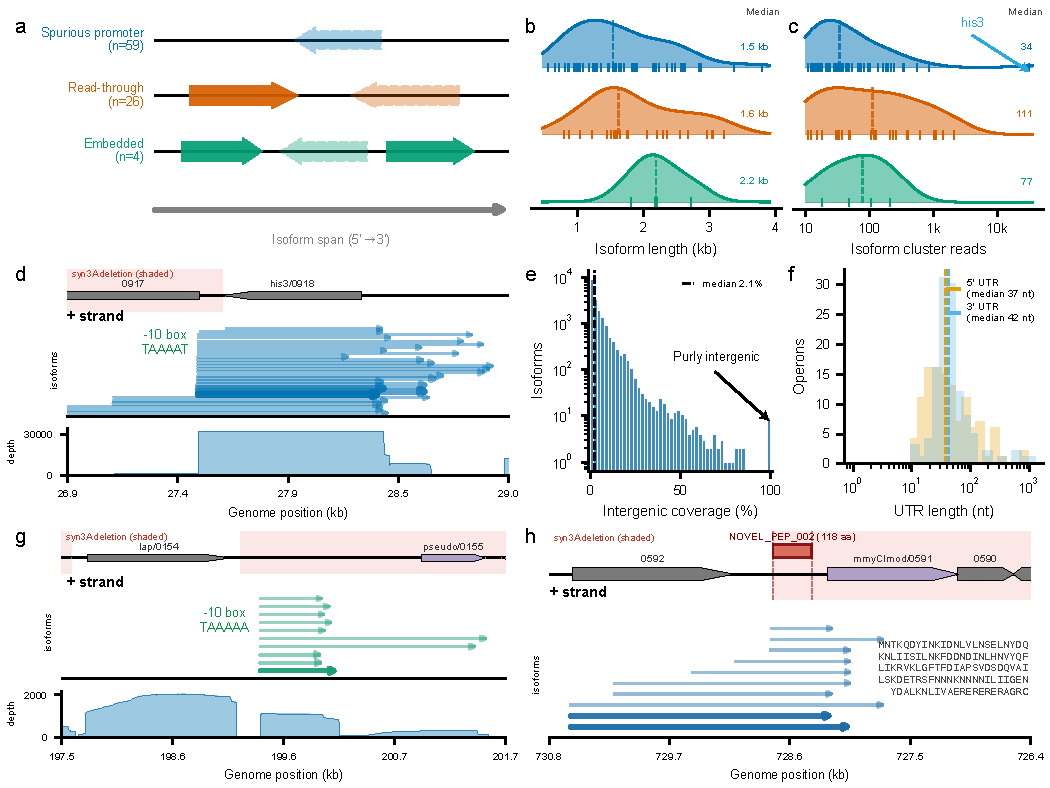
\includegraphics[width=1\linewidth]{figures/novel.pdf}
    \caption{\textbf{Non-canonical transcription and translation in \syn.}
    (a) The three classes of antisense transcription, spurious promoter, read-through, and embedded, relative to the sense isoform span.
    (b) Isoform length and (c) cluster-read support for each class, with the median marked.
    (d) Antisense transcription of the yeast marker \gene{his3}{0918}: gene track, antisense isoforms, and read depth, with the shaded band marking sequence deleted in \syna.
    (e) Distribution of the intergenic coverage fraction across all isoforms.
    (f) \fiveprime~and \threeprime~untranslated-region lengths of canonical operons.
    (g) An isolated intergenic transcript between \gene{lap}{0154} and \locus{0155}.
    (h) A novel 118-amino-acid ORF near \locus{0592} with its covering isoforms and peptide sequence.}
    \label{fig:novel}
\end{figure}
